%%%%%%%%%%%%%%%%%%%%%%%%%%%%%%%%%%%%%%%%%%%%%%%%%%%%%%%%%%%%%%%%%%%%%%%%%%%%%%%
\documentclass[hyperref={pdfpagelabels=false},compress,table]{beamer} % 在Mac下无法编译
% \documentclass[compress,table]{beamer} % 在Mac下使用
% package for font
\usepackage{fontspec}
\defaultfontfeatures{Mapping=tex-text}  %%如果没有它,会有一些 tex 特殊字符无法正常使用,比如连字符。
\usepackage{xunicode,xltxtra}
\usepackage[BoldFont,SlantFont,CJKnumber,CJKchecksingle]{xeCJK}  % \CJKnumber{12345}: 一万二千三百四十五
\usepackage{CJKfntef}  %%实现对汉字加点、下划线等。
\usepackage{pifont}  % \ding{}
% package for math
\usepackage{amsfonts}

% package for graphics
\usepackage[americaninductors,europeanresistors]{circuitikz}
\usepackage{tikz}
\usetikzlibrary{plotmarks}  % placements=positioning
\usepackage{graphicx}  % \includegraphics[]{}
\usepackage{subfigure}  %%图形或表格并排排列
% package for table
\usepackage{colortbl,dcolumn}  %% 彩色表格
\usepackage{multirow}
\usepackage{multicol}
\usepackage{booktabs}
% package for code
\usepackage{fancyvrb}
\usepackage{listings}

% \usepackage{animate}
% \usepackage{movie15}

%%%%%
% setting for beamer
\usetheme{default} % Madrid(常用), Copenhagen, AnnArbor, boxes(白色), Frankfurt,Berkeley
\useoutertheme[subsection=true]{miniframes} % 使用Berkeley时注释本行
\usecolortheme{sidebartab}
\usefonttheme{serif}  %%英文使用衬线字体
% \setbeamertemplate{background canvas}[vertical
% shading][bottom=white,top=structure.fg!7] %%背景色,上25%的蓝,过渡到下白。
\setbeamertemplate{theorems}[numbered]
\setbeamertemplate{navigation symbols}{}  %% 去掉页面下方默认的导航条
\setbeamercovered{transparent}  %设置 beamer 覆盖效果

% 设置标题title背景色
% \setbeamercolor{title}{fg=black, bg=lightgray!60!white}
\setbeamercolor{title}{fg=white, bg=black!70!white}

% 设置每页小LOGO
\pgfdeclareimage[width=1cm]{ouc}{figures/static/ouc.pdf}
\logo{\pgfuseimage{ouc}{\vspace{-20pt}}}

% setting for font
%%\setCJKmainfont{Adobe Kaiti Std}
\setCJKmainfont{SimSun} 
%% \setCJKmainfont{FangSong_GB2312} 
%% \setmainfont{Apple Garamond}  %%苹果字体没有SmallCaps
\setCJKmainfont{SimSun} 
%FUNNY%\setCJKmainfont{DFPShaoNvW5-GB}  %%华康少女文字W5(P)
%FUNNY%\setCJKmainfont{FZJingLeiS-R-GB}  %%方正静蕾体
%FUNNY%\setmainfont{Purisa}
%\setsansfont[Mapping=tex-text]{Adobe Song Std}
     %如果装了Adobe Acrobat,可在font.conf中配置Adobe字体的路径以使用其中文字体。
     %也可直接使用系统中的中文字体如SimSun、SimHei、微软雅黑等。
     %原来beamer用的字体是sans family;注意Mapping的大小写,不能写错。
     %设置字体时也可以直接用字体名,以下三种方式等同:
     %\setromanfont[BoldFont={黑体}]{宋体}
     %\setromanfont[BoldFont={SimHei}]{SimSun}
     %\setromanfont[BoldFont={"[simhei.ttf]"}]{"[simsun.ttc]"}
% setting for graphics
\graphicspath{{figures/}}  %%图片路径
\renewcommand\figurename{图}

% setting for pdf
\hypersetup{% pdfpagemode=FullScreen,%
            pdfauthor={Xiaodong Wang},%
            pdftitle={Title},%
            CJKbookmarks=true,%
            bookmarksnumbered=true,%
            bookmarksopen=false,%
            plainpages=false,%
            colorlinks=true,%
            citecolor=green,%
            filecolor=magenta,%
            linkcolor=blue,%red(default)
            urlcolor=cyan}

% setting for fontspec
\XeTeXlinebreaklocale "zh"  %%表示用中文的断行
\XeTeXlinebreakskip = 0pt plus 1pt minus 0.1pt  %%多一点调整的空间
%%%%%

% font setting by xeCJK
\setCJKfamilyfont{NSimSun}{NSimSun}
\newcommand{\song}{\CJKfamily{NSimSun}}
%%%\setCJKfamilyfont{AdobeSongStd}{Adobe Song Std}
%%%\newcommand{\AdobeSong}{\CJKfamily{AdobeSongStd}}
\setCJKfamilyfont{FangSong}{FangSong_GB2312}
\newcommand{\fang}{\CJKfamily{FangSong}}
%%%\setCJKfamilyfont{AdobeFangsongStd}{Adobe Fangsong Std}
%%%\newcommand{\AdobeFang}{\CJKfamily{AdobeFangsongStd}}
\setCJKfamilyfont{SimHei}{SimHei}
\newcommand{\hei}{\CJKfamily{SimHei}}
%%%\setCJKfamilyfont{AdobeHeitiStd}{Adobe Heiti Std}
%%%\newcommand{\AdobeHei}{\CJKfamily{AdobeHeitiStd}}
\setCJKfamilyfont{KaiTi}{KaiTi}
\newcommand{\kai}{\CJKfamily{KaiTi}}
%%%\setCJKfamilyfont{AdobeKaitiStd}{Adobe Kaiti Std}
\newcommand{\AdobeKai}{\CJKfamily{AdobeKaitiStd}}
\setCJKfamilyfont{LiSu}{LiSu}
\newcommand{\li}{\CJKfamily{LiSu}}
\setCJKfamilyfont{YouYuan}{YouYuan}
\newcommand{\you}{\CJKfamily{YouYuan}}
\setCJKfamilyfont{FZJingLei}{FZJingLeiS-R-GB}
\newcommand{\jinglei}{\CJKfamily{FZJingLei}}
\setCJKfamilyfont{MSYH}{Microsoft YaHei}
\newcommand{\msyh}{\CJKfamily{MSYH}}

% 自定义颜色
\def\Red{\color{red}}
\def\Green{\color{green}}
\def\Blue{\color{blue}}
\def\Mage{\color{magenta}}
\def\Cyan{\color{cyan}}
\def\Brown{\color{brown}}
\def\White{\color{white}}
\def\Black{\color{black}}

\lstnewenvironment{xmlCode}[1][]{% for Java
  \lstset{
    basicstyle=\tiny\ttfamily,%
    columns=flexible,%
    framexleftmargin=.7mm, %
    % frame=shadowbox,%
    % rulesepcolor=\color{cyan},%
     frame=single,%
    backgroundcolor=\color{white},%
    xleftmargin=4\fboxsep,%
    xrightmargin=4\fboxsep,%
    numbers=left,numberstyle=\tiny,%
    numberblanklines=false,numbersep=7pt,%
    language=xml, %
    }\lstset{#1}}{}

\lstnewenvironment{javaCode}[1][]{% for Java
  \lstset{
    basicstyle=\tiny\ttfamily,%
    columns=flexible,%
    framexleftmargin=.7mm, %
    frame=shadowbox,%
    rulesepcolor=\color{cyan},%
    % frame=single,%
    backgroundcolor=\color{white},%
    xleftmargin=4\fboxsep,%
    xrightmargin=4\fboxsep,%
    numbers=left,numberstyle=\tiny,%
    numberblanklines=false,numbersep=7pt,%
    language=Java, %
    }\lstset{#1}}{}

\lstnewenvironment{shCode}[1][]{% for Java
  \lstset{
    basicstyle=\scriptsize\ttfamily,%
    columns=flexible,%
    framexleftmargin=.7mm, %
    frame=shadowbox,%
    rulesepcolor=\color{brown},%
    % frame=single,%
    backgroundcolor=\color{white},%
    xleftmargin=4\fboxsep,%
    xrightmargin=4\fboxsep,%
    numbers=left,numberstyle=\tiny,%
    numberblanklines=false,numbersep=7pt,%
    language=sh, %
    }\lstset{#1}}{}

\newcommand\ask[1]{\vskip 4bp \tikz \node[rectangle,rounded corners,minimum size=6mm,
  fill=white,]{\Cyan \includegraphics[height=1.5cm]{question} \Large \msyh #1};}

\newcommand\wxd[1]{\vskip 4bp \tikz \node[rectangle,minimum size=6mm,
  fill=blue!60!white,]{\White \ding{118} \msyh #1};}

\newcommand\xyy[1]{\vskip 2bp \tikz \node[rectangle,minimum size=3mm,
  fill=black!80!white,]{\White \msyh\scriptsize #1};}

\newcommand\cxf[1]{\vskip 4bp \tikz \node[rectangle,rounded corners,minimum size=6mm,
  fill=orange!60!white,]{\White \ding{42} \msyh #1};}

\newcommand\samp[1]{\vskip 2bp \tikz \node[rectangle,minimum size=3mm,
  fill=white!100!white,]{\Mage\msyh \small CODE \ding{231} \Black #1};\vskip -8bp}

\newcommand\zhyfly[1]{\tikz \node[rectangle,rounded corners,minimum size=6mm,ball color=red!25!blue,text=white,]{#1};}

\setbeamerfont{frametitle}{series=\msyh} % 修改Beamer标题字体

\makeatletter
\newcommand{\Extend}[5]{\ext@arrow 0099{\arrowfill@#1#2#3}{#4}{#5}}
\makeatother


%%%%%%%%%%%%%%%%%%%%%%%%%%%%%%%%%%%%%%%%%%%%%%%%%%%%%%%%%%%%%%%%%%%%%%%%%%%%%%%
% \titlepage
\title[KevinW@OUC]{\hei {\huge Java 应用与开发}\\  
  异常处理}
\author[王晓东]{王晓东\\
  \href{mailto:wangxiaodong@ouc.edu.cn}{\footnotesize wangxiaodong@ouc.edu.cn}}
\institute[中国海洋大学]{\small 中国海洋大学}
\date{\today}
\titlegraphic{\vspace{-6em}
\includegraphics[height=6cm]{static/ouc.pdf}\vspace{-6em}}
%%%%%
\begin{document}
%% Delete this, if you do not want the table of contents to pop up at
%% the beginning of each subsection:
\AtBeginSection[]{                              % 在每个Section前都会加入的Frame
  \frame<handout:0>{
    \frametitle{\textbf{\hei 接下来…}}
    \tableofcontents[currentsection]
  }
}  %

\AtBeginSubsection[]                            % 在每个子段落之前
{
  \frame<handout:0>                             % handout:0 表示只在手稿中出现
  {
    \frametitle{\textit{\hei 接下来…}}\small
    \tableofcontents[current,currentsubsection] % 显示在目录中加亮的当前章节
  }
}
\frame{\titlepage}
%%%%%%%%%%%%%%%%%%%%%%%%%%%%%%%%%%%%%%%%%%%%%%%%
\begin{frame}
  \frametitle{学习目标}
  \begin{enumerate}
  \item 掌握Java异常的概念和分类
  \item 深入理解Java异常处理机制
  \end{enumerate}  
\end{frame}

\section*{大纲}
\frame{\frametitle{大纲} \tableofcontents }


\section{异常的概念及分类}
\begin{frame}[fragile] % [fragile]参数使得能够插入代码
  \frametitle{什么是异常}

  在Java语言中,程序运行出错被称为出现异常(Exception)。异常
  是{\hei\Blue 程序运行过程}中发生的事件,该事件可以中断程序指令的正常执
  行流程。

  \tta{Java异常分为两大类}

  \begin{enumerate}[<+-|alert@+>]\kai
  \item {\hei 错误(Error)}是指JVM系统内部错误、资源耗尽等严重情况。
  \item {\hei 违例(Exception)}则是指其他因编程错误或偶然的外在因素导致
    的一般性问题,例如对负数开平方根、空指针访问、试图读取不存在的文件以
    及网络连接中断等。
  \end{enumerate}

  \notice{小示例} \codeset{sample.exception.FirstExceptionSample.java}
\end{frame}

\begin{frame}[fragile] % [fragile]参数使得能够插入代码
  \frametitle{Java异常分类}

  {\hei\Red Throwable类是Java语言中所有异常类的父类。}

  \begin{figure}
    \centering
    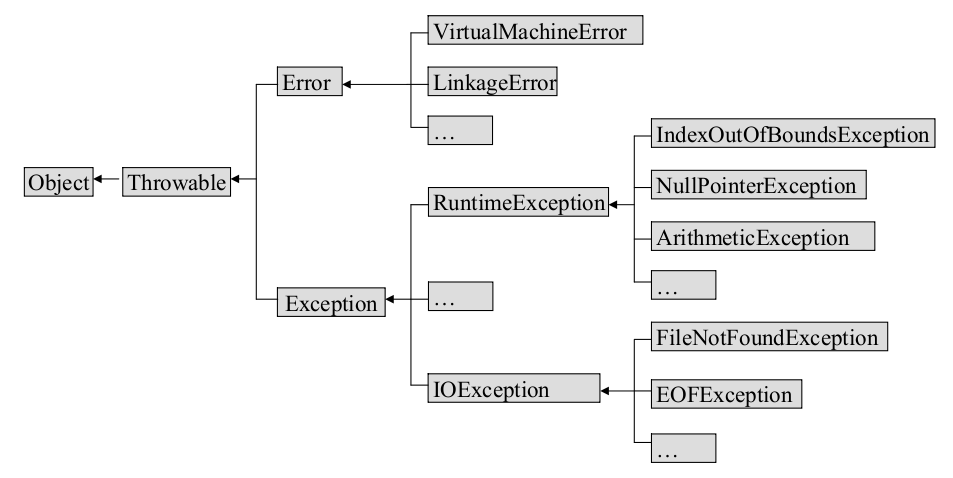
\includegraphics[width=0.95\textwidth]{fig-exception-class.png}
  \end{figure}
\end{frame}

\begin{frame}[fragile] % [fragile]参数使得能够插入代码
  \frametitle{常见错误}

  \tta{链接错误(LinkageError)}

  是指程序链接错误。{\kai 例如,一个类中用到另外一个类,在编译前一个类
    之后,后一个类发生了不相容的改变时,再使用前一个类则会出现链接错误。
    最常见的就是后一个类的.class文件被误删除。}

  \pause

  \tta{虚拟机错误(VirtualMachineError)}

  当Java虚拟机崩溃或资源耗尽时会抛出该错误。其中比较有代表性的
  是StackOverflowError,当应用程序递归太深而导致栈内存溢出时会出现该异
  常。

  \codeset{sample.exception.VMErrorSample.java}

\end{frame}

\begin{frame}[fragile] % [fragile]参数使得能够插入代码
  \frametitle{常见异常}
  
  \tta{RuntimeException}
  
  \begin{itemize}
  \item 错误的类型转换
  \item 数组下标越界
  \item 空指针访问
  \end{itemize}

  \ttc{空指针异常(NullPointerException)}

  如果试图访问不指向任何对象的引用变量的成员,将会产生空指针异常。
  
  \begin{javaCode}
    Person p = null;
    System.out.println(p.age);  
  \end{javaCode}
  
\end{frame}

\begin{frame}[fragile] % [fragile]参数使得能够插入代码
  \frametitle{常见异常}

  \tta{IOException}
  
  \begin{itemize}
  \item 从一个不存在的文件中读取数据
  \item 越过文件结尾继续读取
  \item 连接一个不存在的URL
  \end{itemize}

  \notice{IOException示例}\footnote{{\kai\Red 上述代码无法编译:只要是有可能出现IOException的Java代码,在
    编译时就会出错,而不会等到运行时才发生。}}
  \codeset{sample.exception.IOExceptionSample.java}

\end{frame}

\section{Java异常处理机制}

\begin{frame}[fragile] % [fragile]参数使得能够插入代码
  \frametitle{Java异常处理的原则}

  \begin{itemize}
  \item 返回到一个安全和已知的状态
  \item 能够使用户执行其他的命令
  \item 如果可能,则保存所有的工作
  \item 如果有必要,可以退出以避免造成进一步的危害
  \end{itemize}
\end{frame}

\begin{frame}[fragile] % [fragile]参数使得能够插入代码
  \frametitle{Java异常处理机制}

  \begin{itemize}[<+-|alert@+>]\kai
  \item Java程序执行过程中如出现异常,系统会监测到并自动生成一个相应的
    异常类对象,然后再将它交给运行时系统。
  \item 运行时系统再寻找相应的代码来处理这一异常。如果Java运行时系统找
    不到可以处理异常的代码,则运行时系统将终止,相应的Java程序也将退
    出。
  \item 程序员通常对错误(Error)无能为力,因而一般只处理违
    例(Exception)。
  \end{itemize}
\end{frame}

\begin{frame}[fragile] % [fragile]参数使得能够插入代码
  \frametitle{异常处理结构}

  \tta{异常处理结构}

  \begin{javaCode}
    try {
      ... //可能产生异常的代码,试图捕获异常
      
    } catch (ExceptionName1 e) {
      ... //当产生 ExceptionName1 型异常时的处置措施
      
    } catch (ExceptionName2 e) {
      ... //当产生 ExceptionName2 型异常时的处置措施
      
    } finally {
      ... //无条件执行的语句
      
    }
  \end{javaCode}

  \codeset{sample.exception.HandleFirstExceptionSample.java}

\end{frame}

\begin{frame}[fragile] % [fragile]参数使得能够插入代码
  \frametitle{使用finally语句}

  \begin{itemize}
  \item finally语句是可选的
  \item 作用是为异常处理提供一个统一的出口,使得在控制流转到程序的其他部
    分以前,能够对程序的状态作统一的管理。
  \item 不论try代码块中是否发生了异常事件,finally块中的语句都会被执行。
    当catch语句块中出现return语句时,finally语句块同样会执行。
  \end{itemize}
\end{frame}

\begin{frame}[fragile] % [fragile]参数使得能够插入代码
  \frametitle{操作异常对象}

  发生异常时,系统将自动创建异常类对象,并将作为实参传递给匹配的catch语句
  块的形参,这样就可以在语句块中操纵该异常对象。

  \pause
  
  \tta{异常类的父类Throwable中定义的方法}

  \begin{description}
  \item[getMessage()] 返回描述当前异常的详细消息字符串。
  \item[printStackTrace()] 用来跟踪异常事件发生时运行栈的内容,并将相关
    信息输出到标准错误输出设备。本方法比较常用,在没有找到适合的异常处
    理代码时,系统也会自动调用该方法输出错误信息。
  \end{description}
\end{frame}

%%%%\begin{frame}[fragile] % [fragile]参数使得能够插入代码
%%%%\frametitle{追踪运行栈信息}
%%%%\samp{A.java}
%%%%\begin{javaCode}
%%%%public class A {
%%%%  public void work(int[] a) {
%%%%    String s = this.contain(a, 3);
%%%%    System.out.println("Result: " + s);
%%%%  }
%%%%
%%%%  public String contain(int[] source, int dest) {
%%%%    String result = "no!";
%%%%    try {
%%%%      for (int i = 0; i < source.length; i++) {
%%%%        if (source[i] == dest)
%%%%        result = "yes!";
%%%%      }
%%%%    } catch(Exception e) {
%%%%      System.out.println("异常信息:" + e.getMessage());
%%%%      System.out.println("运行栈信息:");
%%%%      e.printStackTrace();
%%%%      result = "error!";
%%%%    }
%%%%    return result;
%%%%  }
%%%%}
%%%%\end{javaCode}
%%%%\end{frame}
%%%%
%%%%\begin{frame}[fragile] % [fragile]参数使得能够插入代码
%%%%\frametitle{追踪运行栈信息}
%%%%
%%%%\samp{MyTest.java}
%%%%\begin{javaCode}
%%%%public class MyTest {
%%%%  public static void main(String[] args) {
%%%%    A tst = new A();
%%%%    tst.work(null);
%%%%  }
%%%%}
%%%%\end{javaCode}
%%%%
%%%%程序输出结果为:
%%%%\begin{stdoutCode}
%%%%Exception Message: null
%%%%Stack Trace:
%%%%java.lang.NullPointerException
%%%%    at A.contain(A.java:9)
%%%%    at A.work(A.java:3)
%%%%    at MyTest.main(MyTest.java:4)
%%%%Result: error!
%%%%\end{stdoutCode}
%%%%\end{frame}

\begin{frame}[fragile] % [fragile]参数使得能够插入代码
\frametitle{捕获和处理IOException}

\tta{一些知识点}

\begin{itemize}[<+-|alert@+>]\kai
\item {\hei 异常类型的多态性} \only<1>{FileNotFoundException是IOException的子类,基于多态性机制,后一
  个catch语句也可以处理FileNotFoundException,因此前一个catch语句块可以
  取消,但这样就无法区分“文件不存在”或其他I/O异常了。}
\item {\hei 运行时异常} \only<2>{对于只可能产生RuntimeException的代码可以不使用try-catch语句进行处
  理,如果对于这些相对安全的代码仍然采用了try语句块的形式,则try后可以
  省略catch语句块或finally语句块,但不能同时省略。}
\item {\hei 过度处理} \only<3>{如果试图捕获和处理代码中根本不可能出现的异常,编译器也会指出这种
  不当行为。}
\end{itemize}

\codeset{sample.exception.IOExceptionSample.java}
\end{frame}

\begin{frame}[fragile] % [fragile]参数使得能够插入代码
  \frametitle{声明抛出异常}

  \tta{声明抛弃异常是Java中处理Exception的第二种方式}

  \begin{itemize}
  \item 一个方法中的代码在运行时可能生成某种异常,但在本方法中不必或者
    不能确定如何处理此类异常时,则可以声明抛弃该异常。
  \item 此时方法中将不对此类异常进行处理,而是由该方法的调用者负责处理。
  \end{itemize}

  \codeset{sample.exception.ThrowsExceptionSample.java}
\end{frame}


\begin{frame}[fragile] % [fragile]参数使得能够插入代码
\frametitle{声明抛出异常}

\tta{采用声明抛出异常的注意事项}

\begin{itemize}
\item 除非事先约定,否则在开发过程中不要在自己编写的方法中采用抛出异常的方式。
\item {\hei\Red 重写方法不允许抛出比被重写方法范围更大的异常类型。}\\
  例如 IOException重写后抛出FileNotFoundException和EOFException被允许,
  而抛出Exception则不被允许。
\end{itemize}
\end{frame}

\begin{frame}[fragile] % [fragile]参数使得能够插入代码
  \frametitle{人工抛出异常}

  Java异常类对象除了在程序运行出错时由系统自动生成并抛出之外,也可根据需要人工创建并抛
  出:
  \begin{javaCode}
    IOException e = new IOException(); // 创建异常类对象
    throw e; // 抛出操作,即将该异常对象提交给Java运行环境
  \end{javaCode}

  被抛出的必须是Throwable或其子类类型的对象,下述语句在编译时会产生语法错误:

  \begin{javaCode}
    throw new String("want to throw");  
  \end{javaCode}

  \codeset{sample.exception.ManualThrowExceptionSample.java}
\end{frame}

\begin{frame}[fragile] % [fragile]参数使得能够插入代码
\frametitle{人工抛出异常}



\tta{选择人工抛出异常的原则}

\begin{itemize}
\item 当明确知道可能出错的地方或能够通过简单的检查而有效防止错误发生,就应该使用if-else语
  句来预防错误发生。
\item 只有当我们无法明确知道错误发生之处或无法完全避免异常,才不得不通过异常处理的方式来
  捕获和处理异常。
\item 自定义的异常类对象只能采用人工方式抛出。(自定义异常有兴趣请自行搜索资料学习)
\end{itemize}
\end{frame}

%%%%\section{用户自定义异常}
%%%%\begin{frame}[fragile] % [fragile]参数使得能够插入代码
%%%%\frametitle{用户自定义异常}
%%%%%
%%%%\begin{itemize}
%%%%\item Java语言针对常见异常状况已事先定义了相应的异常类型,并在程序运行出错时由系统自动创
%%%%  建相应异常对象并进行抛出、捕获和处理,因此一般不需要用户人工抛出异常对象或定义新的异常
%%%%  类型,{\Blue 但针对特殊的需要也可以这样做。}
%%%%\item 一般通过{\hei 继承Exception类}来实现异常自定义,由于用户自定义的异常不会由系统自动
%%%%  检测并抛出,所以只能靠人工触发并抛出。
%%%%\end{itemize}
%%%%%
%%%%\end{frame}
%%%%
%%%%\begin{frame}[fragile] % [fragile]参数使得能够插入代码
%%%%\frametitle{用户自定义异常}
%%%%%
%%%%\samp{MyException.java}
%%%%\begin{javaCode}
%%%%public class MyException extends Exception {
%%%%  private int idnumber;
%%%%  public MyException(String message, int id) {
%%%%    super(message);
%%%%    this.idnumber = id;
%%%%  }
%%%%  public int getId() {
%%%%    return idnumber;
%%%%  }
%%%%}
%%%%\end{javaCode} 
%%%%
%%%%{\Cyan \small 构造方法中使用super调用其父类Exception的有参构造方法,以在创建异常对象时将
%%%%  用户的定制的报错信息传递给父类中定义的private属性Message(该属性由Throwable类定义),将
%%%%  来在捕获和处理异常时就可以通过调用该对象的getMessage()方法访问到该信息了。}
%%%%%
%%%%\end{frame}
%%%%
%%%%\begin{frame}[fragile] % [fragile]参数使得能够插入代码
%%%%\frametitle{用户自定义异常}
%%%%%
%%%%\samp{TestCustomizingException.java}
%%%%\begin{javaCode}
%%%%public class TestCustomizingException {
%%%%  public void regist(int num) throws MyException {
%%%%    if (num < 0) {
%%%%      throw new MyException("人数为负值,不合理", 3);
%%%%    }
%%%%    System.out.println("登记人数:" + num);
%%%%  }
%%%%  public void manager() {
%%%%    try {
%%%%      regist(-100);
%%%%    } catch (MyException e) {
%%%%      System.out.println("登记失败,出错种类" + e.getId());
%%%%      e.printStackTrace();
%%%%    }
%%%%    System.out.print("本次登记操作结束");
%%%%  }
%%%%  public static void main(String args[]) {
%%%%    new TestCustomizingException().manager();
%%%%  }
%%%%}
%%%%\end{javaCode}
%%%%程序输出结果:
%%%%\begin{stdoutCode}
%%%%登记失败,出错种类3
%%%%MyException: 人数为负值,不合理 ...
%%%%\end{stdoutCode}
%%%%%
%%%%\end{frame}

%%%%\section{断言}
%%%%
%%%%\begin{frame}[fragile] % [fragile]参数使得能够插入代码
%%%%\frametitle{断言}
%%%%从JDK1.4版本开始,Java语言中引入了断言(Assert)机制,允许Java开发者在代码中
%%%%加入一些检查语句,主要用于{\Blue 程序调试目的}。
%%%%
%%%%\begin{itemize}
%%%%\item 断言机制在用户定义的boolean表达式(判定条件)结 果为false时抛出一个Error对象,其类
%%%%  型为AssertionError;
%%%%\item 当我们需要在约定的条件不成立时中断当前操作的话,可以使用断言;
%%%%\item 作为Error的一种,断言失败也不需捕获处理或者声明抛出,一旦出现了则终止程序、不必进行
%%%%  补救和恢复。
%%%%\end{itemize}
%%%%\end{frame}
%%%%
%%%%\begin{frame}[fragile] % [fragile]参数使得能够插入代码
%%%%\frametitle{启用和禁用断言}
%%%%
%%%%\tta{开启断言功能}
%%%%
%%%%Java运行时环境默认设置为关闭断言功能,因此在使用断言以前,需要在运行Java程序时先开启
%%%%断言功能。
%%%%\begin{shCode}
%%%%>java -ea MyAppClass  
%%%%\end{shCode}
%%%%或者:
%%%%\begin{shCode}
%%%%>java -enableassertions MyAppClass  
%%%%\end{shCode}
%%%%
%%%%\tta{关闭断言功能}
%%%%\begin{shCode}
%%%%>java -da MyAppClass  
%%%%\end{shCode}
%%%%或者:
%%%%\begin{shCode}
%%%%java -disableassertions MyAppClass  
%%%%\end{shCode}
%%%%\end{frame}
%%%%
%%%%\begin{frame}[fragile] % [fragile]参数使得能够插入代码
%%%%\frametitle{启用和禁用断言}
%%%%\tta{Eclipse IDE开启断言}
%%%%
%%%%在项目上点击右键 \ding{224} Run As \ding{224} Run Configurations \ding{224} Arguments,
%%%%在VM arguments中,加入-enableassertions或-ea即可。
%%%%\end{frame}
%%%%
%%%%\begin{frame}[fragile] % [fragile]参数使得能够插入代码
%%%%\frametitle{使用断言}
%%%%\tta{断言的语法格式\ding{182}}
%%%%\begin{javaCode}
%%%%assert <boolean 表达式>;  
%%%%\end{javaCode}
%%%%\samp{TestAssertion.java}
%%%%\begin{javaCode}
%%%%public class TestAssertion {
%%%%  public static void main(String[] args) {
%%%%    new TestAssertion().process(-12);
%%%%  }
%%%%  public void process(int age) {
%%%%    assert age >= 0;
%%%%    System.out.println("您的年龄:" + age);
%%%%    // ---
%%%%  }
%%%%}
%%%%\end{javaCode}
%%%%\begin{stdoutCode}
%%%%Exception in thread "main" java.lang.AssertionError
%%%%	at TestAssertion.process(TestAssertion.java:8)
%%%%	at TestAssertion.main(TestAssertion.java:4)  
%%%%\end{stdoutCode}
%%%%\end{frame}
%%%%
%%%%\begin{frame}[fragile] % [fragile]参数使得能够插入代码
%%%%\frametitle{使用断言}
%%%%\tta{断言的语法格式\ding{183}}
%%%%\begin{javaCode}
%%%%assert < boolean 表达式 >:< 表达式 2 >;  
%%%%\end{javaCode}
%%%%\samp{TestAssertion2.java}
%%%%
%%%%\begin{javaCode}
%%%%public class TestAssertion2 {
%%%%  public static void main(String[] args) {
%%%%    new TestAssertion2().process(-12);
%%%%  }
%%%%  public void process(int age) {
%%%%    assert age >= 0: "年龄值不合理";
%%%%    System.out.println("您的年龄:" + age);
%%%%    //---
%%%%  }
%%%%}
%%%%\end{javaCode}
%%%%输出结果:
%%%%\begin{stdoutCode}
%%%%Exception in thread "main" java.lang.AssertionError: 年龄值不合理
%%%%	at TestAssertion.process(TestAssertion.java:8)
%%%%	at TestAssertion.main(TestAssertion.java:4)  
%%%%\end{stdoutCode}
%%%%\end{frame}
%%%%
%%%%\begin{frame}[fragile] % [fragile]参数使得能够插入代码
%%%%\frametitle{使用断言}
%%%%{\small \Cyan 断言失败时,系统会自动将表达式2的值传递给新创建的AssertionError对象,进而将
%%%%  其转换为一个消息字符串保存起来,这样就可以在获得更多/更有针对性的检查失败细节信息。因
%%%%  此,其中的表达式2可以是任何基本数据类型或引用数据类型,但必须提供一个值,即不能
%%%%  为void值。}
%%%%
%%%%{\Red 使用断言是为了在测试阶段确定程序内部出错位置和出错信息,而不是控制程序流程。}
%%%%\end{frame}

\begin{frame}
  \frametitle{本节习题}
  \begin{enumerate}
  \item 总结Java的异常处理机制。
  \item 什么是运行时异常?
  \item 若try语句结构中有多个catch()子句,这些子句的排列顺序与程序执行效果是否有关?
  \item 总结Java异常处理机制随Java版本的更新不断加入的新特性,并附参考文献或网站链接。(选做)
  \end{enumerate}
\end{frame}
%%%%%%%%%%%%%%%%%%%%%%%%%%%%%%%%%%%%%%%%%%%%%%%%%%%%%%%%%%%%%%%%%%%%%%%%%%%%%%%
% TKS Page %%%%%%%%%%%%%%%%%%%%%%%%%%%%%%%%%%%%%%%%%%%%
\begin{frame}
\centering
{\Huge \textcolor{blue}{THE END}} \\
\vspace{5mm}
{\Large wangxiaodong@ouc.edu.cn} \\
\end{frame}
%%%%%%%%%%%%%%%%%%%%%%%%%%%%%%%%%%%%%%%%%%%%%%%%%%%%%%%
%%%%%%%%%%%%%%%%%%%%%%%%%%%%%%%%%%%%%%%%%%%%%%%%%%%%%%%%%%%%%%%%%%%%%%%%%%%%%%%
\end{document}
